%\documentclass[t]{beamer} 
%\hypersetup{pdfpagemode=FullScreen}
\usepackage{indentfirst}
%\usepackage{beamerthemesplit}

\usepackage{makeidx}
%\usepackage[dvipdfm,CJKbookmarks,bookmarks=true,bookmarksnumbered=true]{hyperref}
%\usepackage[CJKbookmarks,bookmarks=true,bookmarksnumbered=true]{hyperref}
\usepackage{listings}
\usepackage{lstlinebgrd}

\usepackage{adjustbox}
\usepackage{dashbox}
\usepackage{mdframed}


% Reduce the space between caption and figure.
\usepackage[skip=2pt]{caption}

\hypersetup{colorlinks, linkcolor=blue, citecolor=blue,
    urlcolor=blue,
    plainpages=flase,
    pdfcreator=tex,
    bookmarksopen=true,
    pdfhighlight=/P,
    pdfauthor={Yao Qi <yao.qi@arm.com>},
    pdfcreator={cTeX},
%    pdftitle={iptables 入门},
%    pdfkeywords={iptables 入门 Rae szlug},
    pdfstartview=FitH,
    pdfpagemode=UseOutlines,%UseOutlines, %None, FullScreen, UseThumbs
}

\usepackage{verbatim} % used to display code
%\usepackage[all,bottom]{draftcopy}
%\draftcopyName{Copyright by Rae <crquan@gmail.com>, 2006}{50}
%\draftcopySetGrey{0.8} \draftcopyPageTransform{55 rotate}
%\draftcopyPageX{80}\draftcopyPageY{-25}

\usepackage{caption}
\captionsetup[lstlisting]{font={small}}


\usepackage{xcolor}

\lstset{
  basicstyle=\ttfamily,          % print whole listing small
  showstringspaces=false,
  %backgroundcolor = \color{lightgray},
  xrightmargin=3ex,
  xleftmargin=3ex,
  %numbers=left,
  %numberstyle=\tiny,
  % labelstep=1,
  commentstyle=\textsl,
  keywordstyle=\color{blue}\bfseries\underbar,     % underlined bold red keywords
  keywordstyle = [2]{\color{lime}},
  keywordstyle = [3]{\color{yellow}},
  keywordstyle = [4]{\color{teal}},
  identifierstyle={\color{black}\textbf}, % nothing happens to other identifiers
  commentstyle=\mdseries\color{magenta}, % white comments
  captionpos=b,
  otherkeywords={NULL,?,:},
  morekeywords = [2]{NULL,?,:},
  %morekeywords = [3]{\[, \]},
  emph={int,char,void,long,bool,target\_desc,true,false,X86\_XSTATE\_AVX512,X86\_XSTATE\_AVX,X86\_XSTATE\_MPX,X86\_XSTATE\_PKRU},
  emphstyle={\color{violet}},
  stringstyle=\color{red}\ttfamily}      % typewriter type for strings
% stringspaces=false}         % no special string spaces



%\usetheme{Madrid}  % theme

%\usetheme{Warsaw}
%\usetheme{Rochester}
%\usetheme{PaloAlto}
%\usetheme{Montpellier}
%\usetheme{Berlin}
%\usetheme{Ilmenau}
%\usetheme{Dresden}

%\usecolortheme{albatross}
%\usecolortheme{beaver} white background
%\usecolortheme{beetle}
%\usecolortheme{dolphin}
%\usecolortheme{fly}
%\usecolortheme{lily}
%\useoutertheme{tree}

%\usefonttheme{structureitalicserif}

\usepackage{array}
\newcounter{rowcount}
\setcounter{rowcount}{0}



% color in each row
\usepackage{tabularx,colortbl}

%\setbeamersize{text margin left=30mm,text margin right=30mm} 
%\usepackage{pgfpages}
%\setbeameroption{show notes on second screen=right}

\usepackage{tikz}
\usetikzlibrary{positioning,arrows,shadows,calc,fit,shapes.geometric}

%\usepackage{enumitem}
%\setlist[itemize]{noitemsep, nolistsep}

\begin{document}


\title{A flexible GDB target description for processor diversity}
% https://www.linkedin.com/pulse/wordpress-rest-api-picnmix-components-your-mobile-app-conor-woods
\titlegraphic{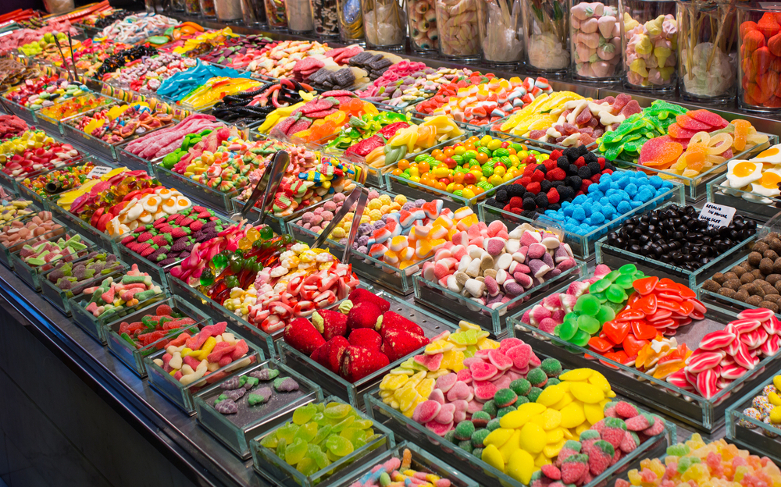
\includegraphics[scale=0.8]{pic/mix_and_match.jpg}}

\author{\href{mailto:yao.qi@arm.com}{Yao Qi}}
\date[20170909]{GNU Cauldron 2017}

%\institute{ARM}
%\logo{\includegraphics[width=30pt]{pic/Arm_logo_blue_72LG.png}}
% 生成上面定义的"\title", "\author", "\date"等信息
\frame{
  \titlepage
  \note{start}
}


% 生成目录菜单
\section{Contents}
\frame{
  \tableofcontents
  \note[item]{Explain what target description is in GDB, its shortcomings,}
  \note[item]{The new design is to address all these shortcomings,}
}

\section{Background}

\subsection{GDB target description}

\begin{frame}[squeeze]{GDB target description}
  \vspace{-2\baselineskip}

  \only<+->

  \begin{columns}[t]
    \begin{column}[t]{0.55\textwidth}

      \begin{itemize}
      \item<+-> GDB asks about the remote target
        \note<.>{When GDB connects to the remote target, it wants to know about the registers, types, etc, so it asks,}
        \only<+->{
        \begin{figure}
          
\includegraphics[scale=0.2]{pic/tell_me_about_yourself.jpg}
        \end{figure}
        }
      \item<+-> Describe architecture variants, their registers and types, in XML,
      \item<+-> Added by Daniel Jacobowitz in 2006,2007,
      \item<.-> Used in many projects, like QEMU, OpenOCD,
      \item<.-> \href{https://sourceware.org/gdb/current/onlinedocs/gdb/Target-Descriptions.html}{Appendix G Target Descriptions}
        \note<.>[item]{Widely used by other projects,}
        \note<.>[item]{GDB manual about target description is quite good,}
      \end{itemize}

    \end{column}

    \begin{column}[t]{0.45\textwidth}
      \only<4->{
      \begin{exampleblock}{Sample target description}
        \begin{adjustbox}{max totalsize={1\textwidth}{1\textheight}, center}
          \lstinputlisting[language=XML,firstline=4]{code/aarch64.xml}
        \end{adjustbox}
      \end{exampleblock}
      \note<4>{Use include other XML files via xi:include,}
      }
    \end{column}
  \end{columns}
\end{frame}

\frame{
  \frametitle{How does target description work?}
  \note<.>[item]{In order to clearly point out the shortcomings of gdb target description, need to know how existing gdb target description works.\\}

  \begin{adjustbox}{max totalsize={1\textwidth}{.5\textheight},center}
    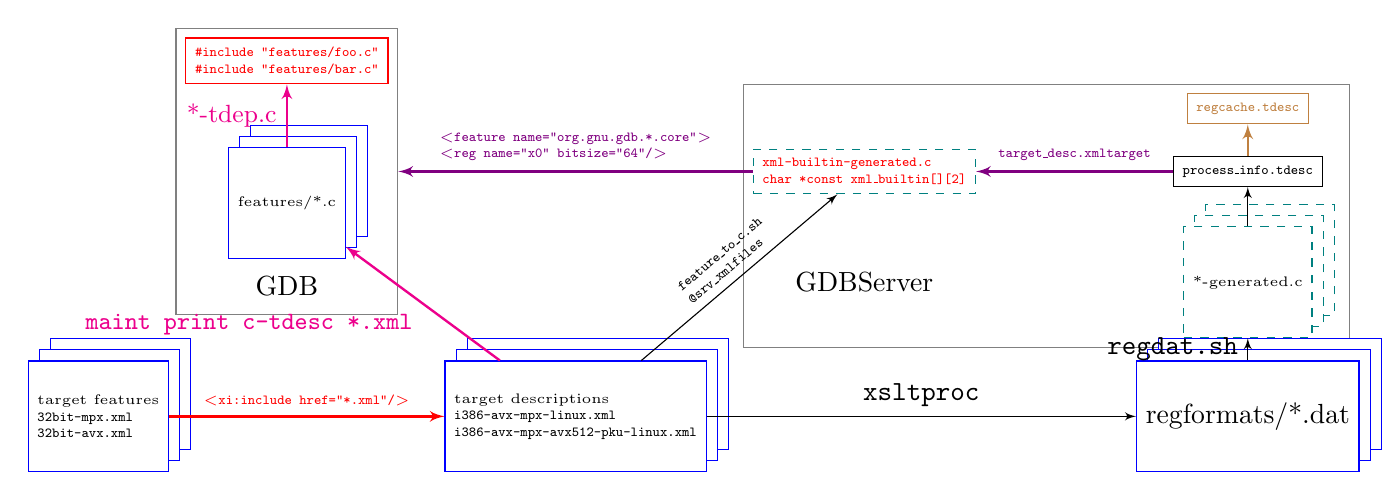
\begin{tikzpicture}[
  auto, >=latex',
  doc/.style={minimum height=4em, minimum width=3em, fill=white, draw=blue, double copy shadow={shadow xshift=4pt, 
      shadow yshift=4pt, fill=white, draw}},
]

  \node (gdb-tdep)[draw, align=left, font=\tiny, color=red] {\texttt{\#include "features/foo.c"}\\\texttt{\#include "features/bar.c"}};
  \node (gdb-features)[below=8mm of gdb-tdep, draw, align=left, doc] {\tiny features/*.c};
  \draw[->,color=magenta,line width=0.3mm] (gdb-features) -- node[align=left] {\small *-tdep.c} (gdb-tdep);
  \node (gdb) [below=1mm of gdb-features] {GDB};
  \node (gdb1) [draw=black!50, fit={(gdb) (gdb-tdep) (gdb-features) ($(gdb-features.south east)+(10pt,0pt)$)}] {};

  % GDBserver
  \node (gdbserver-builtin)[right=4.5cm of gdb1, align=left, draw=teal, dashed, font=\tiny, text=red] {\texttt{xml-builtin-generated.c} \\ \texttt{char *const xml\_builtin[][2]}};

  \node (gdbserver-process)[right=25mm of gdbserver-builtin, draw, align=left] {\tiny\texttt{process\_info.tdesc}};
  \node (gdbserver-generated)[below=5mm of gdbserver-process, align=left, doc, draw=teal, dashed] {\tiny *-generated.c};
  \node (gdbserver) [at=(gdbserver-builtin |- gdbserver-generated)] {GDBServer};
  \draw[->,color=violet,line width=0.3mm] (gdbserver-process) -- node[above,sloped]{\tiny\texttt{target\_desc.xmltarget}} (gdbserver-builtin);

  \node (gdbserver-regcache)[above=4mm of gdbserver-process,draw, align=left,color=brown] {\tiny\texttt{regcache.tdesc}};
  \draw[->] (gdbserver-generated) -- (gdbserver-process);
  \draw[->,color=brown,line width=0.3mm] (gdbserver-process) -- (gdbserver-regcache);
  \node (gdbserver1) [draw=black!50, fit={(gdbserver) (gdbserver-regcache) (gdbserver-process) (gdbserver-builtin) (gdbserver-generated) ($(gdbserver-generated.south east)+(10pt,0pt)$)}] {};
  \draw[->,color=violet,line width=0.3mm] (gdbserver-builtin) -- node[name=xml,align=left,sloped,font=\tiny] {\texttt{\textless feature name="org.gnu.gdb.*.core"\textgreater} \\ \texttt{\textless reg name="x0" bitsize="64"/\textgreater}} (gdb1);

  \node[below=2.4cm of xml, doc,align=left,font=\tiny] (doc) {target descriptions \\ \texttt{i386-avx-mpx-linux.xml} \\ \texttt{i386-avx-mpx-avx512-pku-linux.xml}};
  \node[left=35mm of doc, doc,align=left, anchor=east,font=\tiny] (features) {target features \\ \texttt{32bit-mpx.xml} \\ \texttt{32bit-avx.xml} };
  \draw[->,color=red,line width=0.3mm] (features) -- node {\tiny\texttt{\textless xi:include href="*.xml"/\textgreater}} (doc);

  \node[at=(gdbserver-generated |- doc), doc] (dat) {regformats/*.dat};

  \draw[->] (doc) -- node[above] {\texttt{xsltproc}} (dat);
  \draw[->] (dat) -- node {\texttt{regdat.sh}} (gdbserver-generated);
  \draw[->,color=magenta,line width=0.3mm] (doc) -- node[below, align=left, anchor=north east] {\small\texttt{maint print c-tdesc *.xml}} (gdb-features);
  \draw[->] (doc) -- node[above, align=left, sloped, font=\tiny] {\texttt{feature\_to\_c.sh} \\ \texttt{@srv\_xmlfiles}} (gdbserver-builtin);
\end{tikzpicture}

  \end{adjustbox}

  \note[item]{dotted boxes are generated files,}
  \note[item]{It does three things,}

  \begin{block}{}
    \begin{itemize}
    \item \small\textcolor{violet}{Tells GDB what registers the remote target have, in a format of XML},
      \note[item]{in a format of XML, GDBserver sends the right XML contents for the current process}
    \item \small\textcolor{brown}{GDBserver manages \texttt{regcache} internally},
    \item \small\textcolor{magenta}{Pre-generate some builtin target descriptions used in native debugging},
      \note[item]{even if GDB can't parse XML}
    \end{itemize}
  \end{block}

  \note[item]{start from target features, then target descriptions, then generated files,}
  \note[item]{three major shortcomings, shown in red}

}

\subsection{Shortcomings}
\frame{
  \frametitle{Shortcomings}
  \vspace*{-0.4cm}

  \begin{itemize}
  \item<+->\small target description XML files \texttt{xi:include} target feature XML files.
    \only<.->{
      \begin{adjustbox}{precode=\dbox, max totalsize={.8\textheight},clip=true,trim=0mm 0mm 8.5cm 4.5cm}
        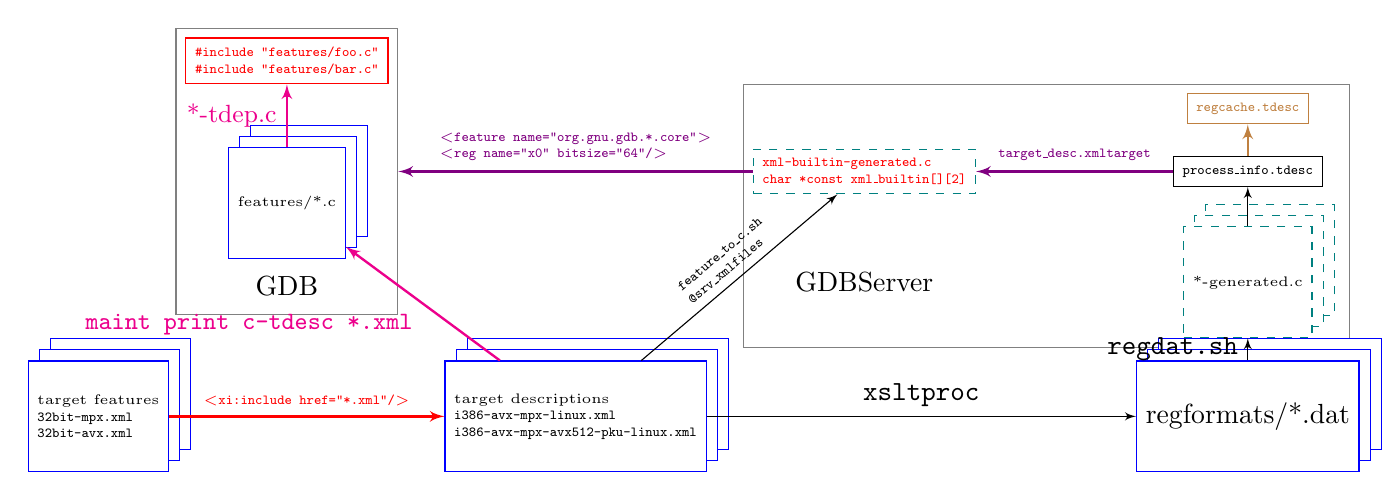
\begin{tikzpicture}[
  auto, >=latex',
  doc/.style={minimum height=4em, minimum width=3em, fill=white, draw=blue, double copy shadow={shadow xshift=4pt, 
      shadow yshift=4pt, fill=white, draw}},
]

  \node (gdb-tdep)[draw, align=left, font=\tiny, color=red] {\texttt{\#include "features/foo.c"}\\\texttt{\#include "features/bar.c"}};
  \node (gdb-features)[below=8mm of gdb-tdep, draw, align=left, doc] {\tiny features/*.c};
  \draw[->,color=magenta,line width=0.3mm] (gdb-features) -- node[align=left] {\small *-tdep.c} (gdb-tdep);
  \node (gdb) [below=1mm of gdb-features] {GDB};
  \node (gdb1) [draw=black!50, fit={(gdb) (gdb-tdep) (gdb-features) ($(gdb-features.south east)+(10pt,0pt)$)}] {};

  % GDBserver
  \node (gdbserver-builtin)[right=4.5cm of gdb1, align=left, draw=teal, dashed, font=\tiny, text=red] {\texttt{xml-builtin-generated.c} \\ \texttt{char *const xml\_builtin[][2]}};

  \node (gdbserver-process)[right=25mm of gdbserver-builtin, draw, align=left] {\tiny\texttt{process\_info.tdesc}};
  \node (gdbserver-generated)[below=5mm of gdbserver-process, align=left, doc, draw=teal, dashed] {\tiny *-generated.c};
  \node (gdbserver) [at=(gdbserver-builtin |- gdbserver-generated)] {GDBServer};
  \draw[->,color=violet,line width=0.3mm] (gdbserver-process) -- node[above,sloped]{\tiny\texttt{target\_desc.xmltarget}} (gdbserver-builtin);

  \node (gdbserver-regcache)[above=4mm of gdbserver-process,draw, align=left,color=brown] {\tiny\texttt{regcache.tdesc}};
  \draw[->] (gdbserver-generated) -- (gdbserver-process);
  \draw[->,color=brown,line width=0.3mm] (gdbserver-process) -- (gdbserver-regcache);
  \node (gdbserver1) [draw=black!50, fit={(gdbserver) (gdbserver-regcache) (gdbserver-process) (gdbserver-builtin) (gdbserver-generated) ($(gdbserver-generated.south east)+(10pt,0pt)$)}] {};
  \draw[->,color=violet,line width=0.3mm] (gdbserver-builtin) -- node[name=xml,align=left,sloped,font=\tiny] {\texttt{\textless feature name="org.gnu.gdb.*.core"\textgreater} \\ \texttt{\textless reg name="x0" bitsize="64"/\textgreater}} (gdb1);

  \node[below=2.4cm of xml, doc,align=left,font=\tiny] (doc) {target descriptions \\ \texttt{i386-avx-mpx-linux.xml} \\ \texttt{i386-avx-mpx-avx512-pku-linux.xml}};
  \node[left=35mm of doc, doc,align=left, anchor=east,font=\tiny] (features) {target features \\ \texttt{32bit-mpx.xml} \\ \texttt{32bit-avx.xml} };
  \draw[->,color=red,line width=0.3mm] (features) -- node {\tiny\texttt{\textless xi:include href="*.xml"/\textgreater}} (doc);

  \node[at=(gdbserver-generated |- doc), doc] (dat) {regformats/*.dat};

  \draw[->] (doc) -- node[above] {\texttt{xsltproc}} (dat);
  \draw[->] (dat) -- node {\texttt{regdat.sh}} (gdbserver-generated);
  \draw[->,color=magenta,line width=0.3mm] (doc) -- node[below, align=left, anchor=north east] {\small\texttt{maint print c-tdesc *.xml}} (gdb-features);
  \draw[->] (doc) -- node[above, align=left, sloped, font=\tiny] {\texttt{feature\_to\_c.sh} \\ \texttt{@srv\_xmlfiles}} (gdbserver-builtin);
\end{tikzpicture}

      \end{adjustbox}
    }

    \tiny{
    \begin{itemize}
    \item<.-> More extensions and variants of computer architecture,
    \item<.-> 3 optional target features can create 7 target descriptions.  What if we have 4, 5 or more optional target features?
    \end{itemize}
    }

    \note<1>[item]{What if we have more target features?}
    \note<.>[item]{Doesn't scale for different combination of target features}
    \note<.>[item]{We've already had XML target features, but we also need XML target descriptions which statically include target features,}

  \item<+-> Inflexible target descriptions: x86
  \end{itemize}

  \only<.->{
    \makebox[.9\textwidth][c]{       %centering table
    \resizebox{.9\textwidth}{!}{   %resize table
      \begin{tabular}{|p{50mm}|p{70mm}|l|} \hline
        commit&files changed or added&\\ \hline
        \tiny \#{\refstepcounter{rowcount}\therowcount\label<2>{row:x86}.} \texttt{4676342} Add x86 XML target description files&\tiny \textcolor{blue}{32bit-core.xml 32bit-linux.xml 32bit-sse.xml 64bit-core.xml 64bit-linux.xml 64bit-sse.xml} \{amd64,i386\}\{-linux,\}.\{xml,c,dat\}&\\ \hline
        \rowcolor{lightgray}\tiny \#{\refstepcounter{rowcount}\therowcount.} \texttt{3a13a53} Support i386 without SSE.&\tiny i386-mmx\{-linux,\}.\{xml,c,dat\}&\tiny \#\ref{row:x86}\\ \hline
        \tiny \#{\refstepcounter{rowcount}\therowcount\label<2>{row:avx}.} \texttt{98adf0f} Add x86 AVX XML files.&\tiny \textcolor{blue}{32bit-avx.xml 64bit-avx.xml} \{amd64,i386\}-avx\{-linux,\}.\{xml,c,dat\}&\\ \hline
        \tiny \#{\refstepcounter{rowcount}\therowcount\label<2>{row:mpx}.} \texttt{ccc42043f} Add MPX registers XML files.&\tiny \textcolor{blue}{32bit-mpx.xml 64bit-mpx.xml} \{amd64,i386\}-mpx\{-linux,\}.\{xml,c,dat\}&\\ \hline
        \tiny \#{\refstepcounter{rowcount}\therowcount\label<2>{row:avx512}.} \texttt{01f9f80} Add AVX512 registers support to GDB and GDBserver.&\tiny \textcolor{blue}{32bit-avx512.xml 64bit-avx512.xml} \newline \{amd64,i386,x32\}-avx512\{-linux,\}.\{xml,c,dat\}&\\ \hline
        \rowcolor{lightgray}\tiny \#{\refstepcounter{rowcount}\therowcount.} \texttt{2b863f5} Add target descriptions for AVX + MPX&\tiny \{amd64,i386\}-avx-mpx\{-linux,\}.\{xml,c,dat\} &\tiny \#\ref{row:avx} and \#\ref{row:mpx}\\ \hline
        \rowcolor{lightgray}\tiny \#{\refstepcounter{rowcount}\therowcount.} \texttt{a1fa17e} Add target description for avx-avx512.&\tiny \{amd64,i386\}-avx-avx512\{-linux\}.\{xml,c,dat\}&\tiny \#\ref{row:avx} and \#\ref{row:avx512}\\ \hline
        \tiny \#{\refstepcounter{rowcount}\therowcount.} \texttt{2735833} amd64-linux: expose system register FS\_BASE and GS\_BASE for Linux.&\tiny \textcolor{blue}{64bit-segments.xml} amd64-\{avx,avx-mpx,avx512,\}-linux.\{xml,c,dat\} x32-\{avx,avx512,\}-linux.\{xml,c,dat\} &\\ \hline
        \tiny \#{\refstepcounter{rowcount}\therowcount.} \texttt{51547df} Add support for Intel PKRU register to GDB and GDBserver&\tiny \textcolor{blue}{32bit-pkeys.xml 64bit-pkeys.xml} \newline \{amd64,i386\}-avx-mpx-avx512-pku\{-linux,\}.\{xml,c,dat\}&\\ \hline
      \end{tabular}
    } %close resize
  } %close centering

  \note<.>[item]{This table is about the commit history about x86 target descriptions,}
  \note<.>[item]{Combine features added by commits \#\ref{row:mpx}, \#\ref{row:avx}, \#\ref{row:avx512}}
}
}

\frame{
  \frametitle{Shortcomings}
  \vspace*{-0.4cm}
  \begin{columns}[t]
    \begin{column}[t]{0.45\textwidth}

        \begin{block}{manually include}

          \only<+->{
            \begin{adjustbox}{max totalsize={.6\textwidth},precode=\dbox,clip=true,
                trim={.05\width} % Trim width from the left
                {.75\height} % Trim height from the bottom
                {0.7\width} % Trim width from the right
                {.01\height}} % Trim height from the top
              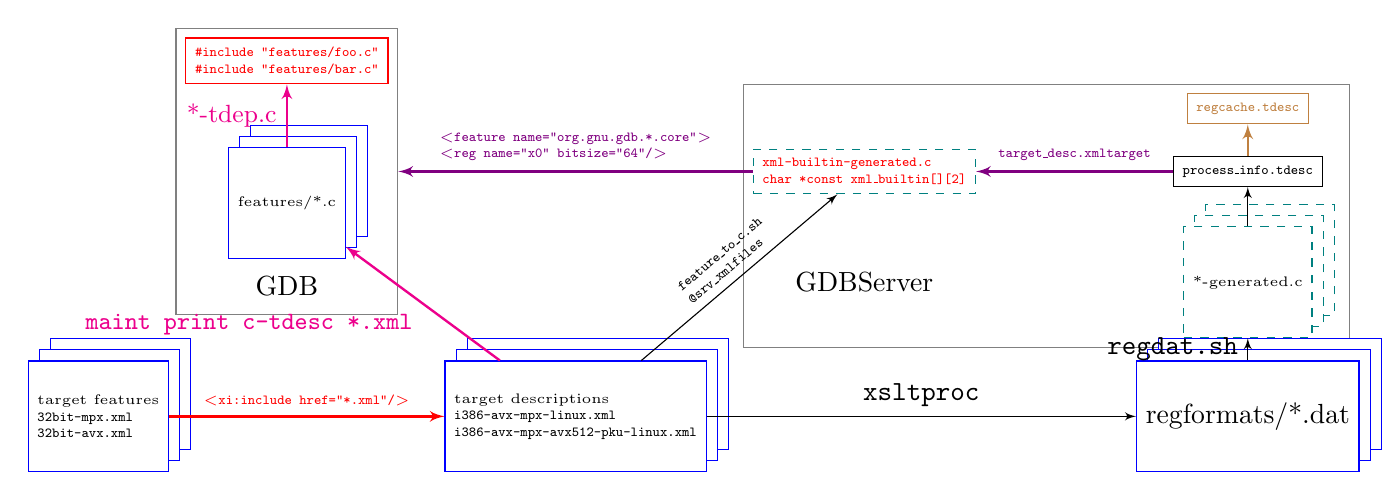
\begin{tikzpicture}[
  auto, >=latex',
  doc/.style={minimum height=4em, minimum width=3em, fill=white, draw=blue, double copy shadow={shadow xshift=4pt, 
      shadow yshift=4pt, fill=white, draw}},
]

  \node (gdb-tdep)[draw, align=left, font=\tiny, color=red] {\texttt{\#include "features/foo.c"}\\\texttt{\#include "features/bar.c"}};
  \node (gdb-features)[below=8mm of gdb-tdep, draw, align=left, doc] {\tiny features/*.c};
  \draw[->,color=magenta,line width=0.3mm] (gdb-features) -- node[align=left] {\small *-tdep.c} (gdb-tdep);
  \node (gdb) [below=1mm of gdb-features] {GDB};
  \node (gdb1) [draw=black!50, fit={(gdb) (gdb-tdep) (gdb-features) ($(gdb-features.south east)+(10pt,0pt)$)}] {};

  % GDBserver
  \node (gdbserver-builtin)[right=4.5cm of gdb1, align=left, draw=teal, dashed, font=\tiny, text=red] {\texttt{xml-builtin-generated.c} \\ \texttt{char *const xml\_builtin[][2]}};

  \node (gdbserver-process)[right=25mm of gdbserver-builtin, draw, align=left] {\tiny\texttt{process\_info.tdesc}};
  \node (gdbserver-generated)[below=5mm of gdbserver-process, align=left, doc, draw=teal, dashed] {\tiny *-generated.c};
  \node (gdbserver) [at=(gdbserver-builtin |- gdbserver-generated)] {GDBServer};
  \draw[->,color=violet,line width=0.3mm] (gdbserver-process) -- node[above,sloped]{\tiny\texttt{target\_desc.xmltarget}} (gdbserver-builtin);

  \node (gdbserver-regcache)[above=4mm of gdbserver-process,draw, align=left,color=brown] {\tiny\texttt{regcache.tdesc}};
  \draw[->] (gdbserver-generated) -- (gdbserver-process);
  \draw[->,color=brown,line width=0.3mm] (gdbserver-process) -- (gdbserver-regcache);
  \node (gdbserver1) [draw=black!50, fit={(gdbserver) (gdbserver-regcache) (gdbserver-process) (gdbserver-builtin) (gdbserver-generated) ($(gdbserver-generated.south east)+(10pt,0pt)$)}] {};
  \draw[->,color=violet,line width=0.3mm] (gdbserver-builtin) -- node[name=xml,align=left,sloped,font=\tiny] {\texttt{\textless feature name="org.gnu.gdb.*.core"\textgreater} \\ \texttt{\textless reg name="x0" bitsize="64"/\textgreater}} (gdb1);

  \node[below=2.4cm of xml, doc,align=left,font=\tiny] (doc) {target descriptions \\ \texttt{i386-avx-mpx-linux.xml} \\ \texttt{i386-avx-mpx-avx512-pku-linux.xml}};
  \node[left=35mm of doc, doc,align=left, anchor=east,font=\tiny] (features) {target features \\ \texttt{32bit-mpx.xml} \\ \texttt{32bit-avx.xml} };
  \draw[->,color=red,line width=0.3mm] (features) -- node {\tiny\texttt{\textless xi:include href="*.xml"/\textgreater}} (doc);

  \node[at=(gdbserver-generated |- doc), doc] (dat) {regformats/*.dat};

  \draw[->] (doc) -- node[above] {\texttt{xsltproc}} (dat);
  \draw[->] (dat) -- node {\texttt{regdat.sh}} (gdbserver-generated);
  \draw[->,color=magenta,line width=0.3mm] (doc) -- node[below, align=left, anchor=north east] {\small\texttt{maint print c-tdesc *.xml}} (gdb-features);
  \draw[->] (doc) -- node[above, align=left, sloped, font=\tiny] {\texttt{feature\_to\_c.sh} \\ \texttt{@srv\_xmlfiles}} (gdbserver-builtin);
\end{tikzpicture}

            \end{adjustbox}

            \small \texttt{*-tdep.c} files have to \texttt{\#include "features/*.c"}

            \begin{adjustbox}{max totalsize={1\textwidth}, left}
              \lstinputlisting[language=C]{code/include-features.c}
            \end{adjustbox}
          }

          \note<.->{has to include all these target description .c files, }
        \end{block}

    \end{column}

    \begin{column}[t]{0.55\textwidth}

      \only<+->{
      \begin{block}{duplication}
        \only<.->{
          \begin{adjustbox}{center, precode=\dbox,clip=true,
            trim={.48\width} % Trim width from the left
            {.65\height} % Trim height from the bottom
            {.25\width} % Trim width from the right
            {.24\height}} % Trim height from the top
            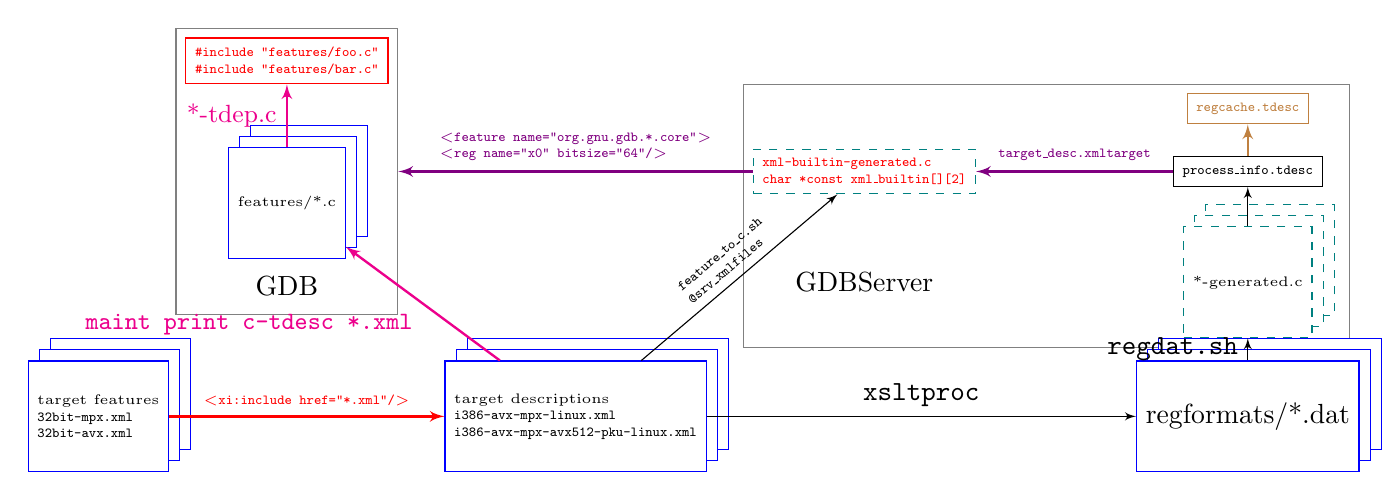
\begin{tikzpicture}[
  auto, >=latex',
  doc/.style={minimum height=4em, minimum width=3em, fill=white, draw=blue, double copy shadow={shadow xshift=4pt, 
      shadow yshift=4pt, fill=white, draw}},
]

  \node (gdb-tdep)[draw, align=left, font=\tiny, color=red] {\texttt{\#include "features/foo.c"}\\\texttt{\#include "features/bar.c"}};
  \node (gdb-features)[below=8mm of gdb-tdep, draw, align=left, doc] {\tiny features/*.c};
  \draw[->,color=magenta,line width=0.3mm] (gdb-features) -- node[align=left] {\small *-tdep.c} (gdb-tdep);
  \node (gdb) [below=1mm of gdb-features] {GDB};
  \node (gdb1) [draw=black!50, fit={(gdb) (gdb-tdep) (gdb-features) ($(gdb-features.south east)+(10pt,0pt)$)}] {};

  % GDBserver
  \node (gdbserver-builtin)[right=4.5cm of gdb1, align=left, draw=teal, dashed, font=\tiny, text=red] {\texttt{xml-builtin-generated.c} \\ \texttt{char *const xml\_builtin[][2]}};

  \node (gdbserver-process)[right=25mm of gdbserver-builtin, draw, align=left] {\tiny\texttt{process\_info.tdesc}};
  \node (gdbserver-generated)[below=5mm of gdbserver-process, align=left, doc, draw=teal, dashed] {\tiny *-generated.c};
  \node (gdbserver) [at=(gdbserver-builtin |- gdbserver-generated)] {GDBServer};
  \draw[->,color=violet,line width=0.3mm] (gdbserver-process) -- node[above,sloped]{\tiny\texttt{target\_desc.xmltarget}} (gdbserver-builtin);

  \node (gdbserver-regcache)[above=4mm of gdbserver-process,draw, align=left,color=brown] {\tiny\texttt{regcache.tdesc}};
  \draw[->] (gdbserver-generated) -- (gdbserver-process);
  \draw[->,color=brown,line width=0.3mm] (gdbserver-process) -- (gdbserver-regcache);
  \node (gdbserver1) [draw=black!50, fit={(gdbserver) (gdbserver-regcache) (gdbserver-process) (gdbserver-builtin) (gdbserver-generated) ($(gdbserver-generated.south east)+(10pt,0pt)$)}] {};
  \draw[->,color=violet,line width=0.3mm] (gdbserver-builtin) -- node[name=xml,align=left,sloped,font=\tiny] {\texttt{\textless feature name="org.gnu.gdb.*.core"\textgreater} \\ \texttt{\textless reg name="x0" bitsize="64"/\textgreater}} (gdb1);

  \node[below=2.4cm of xml, doc,align=left,font=\tiny] (doc) {target descriptions \\ \texttt{i386-avx-mpx-linux.xml} \\ \texttt{i386-avx-mpx-avx512-pku-linux.xml}};
  \node[left=35mm of doc, doc,align=left, anchor=east,font=\tiny] (features) {target features \\ \texttt{32bit-mpx.xml} \\ \texttt{32bit-avx.xml} };
  \draw[->,color=red,line width=0.3mm] (features) -- node {\tiny\texttt{\textless xi:include href="*.xml"/\textgreater}} (doc);

  \node[at=(gdbserver-generated |- doc), doc] (dat) {regformats/*.dat};

  \draw[->] (doc) -- node[above] {\texttt{xsltproc}} (dat);
  \draw[->] (dat) -- node {\texttt{regdat.sh}} (gdbserver-generated);
  \draw[->,color=magenta,line width=0.3mm] (doc) -- node[below, align=left, anchor=north east] {\small\texttt{maint print c-tdesc *.xml}} (gdb-features);
  \draw[->] (doc) -- node[above, align=left, sloped, font=\tiny] {\texttt{feature\_to\_c.sh} \\ \texttt{@srv\_xmlfiles}} (gdbserver-builtin);
\end{tikzpicture}

          \end{adjustbox}
          \small \texttt{xml\_builtin} is a map of all needed XML files (target descriptions and target features) names and contents

          \note[item]<.>{duplication, get gdbserver size bigger, all XML contents are copied into GDBserver}

          \begin{adjustbox}{max totalsize={\textwidth},center}
            \lstinputlisting[language=C]{code/xml-builtin.c}
          \end{adjustbox}
        }
      \end{block}
      }
    \end{column}
    \end{columns}
}

\section{New design}

\subsection{New design}
\frame{
  \frametitle{New design}

  \begin{columns}
    \column[t]{0.5\textwidth}

    \begin{figure}[t]
      \centering
      \vspace*{-1cm}
      \begin{adjustbox}{precode=\dbox, max totalsize={1\textwidth}, center}
        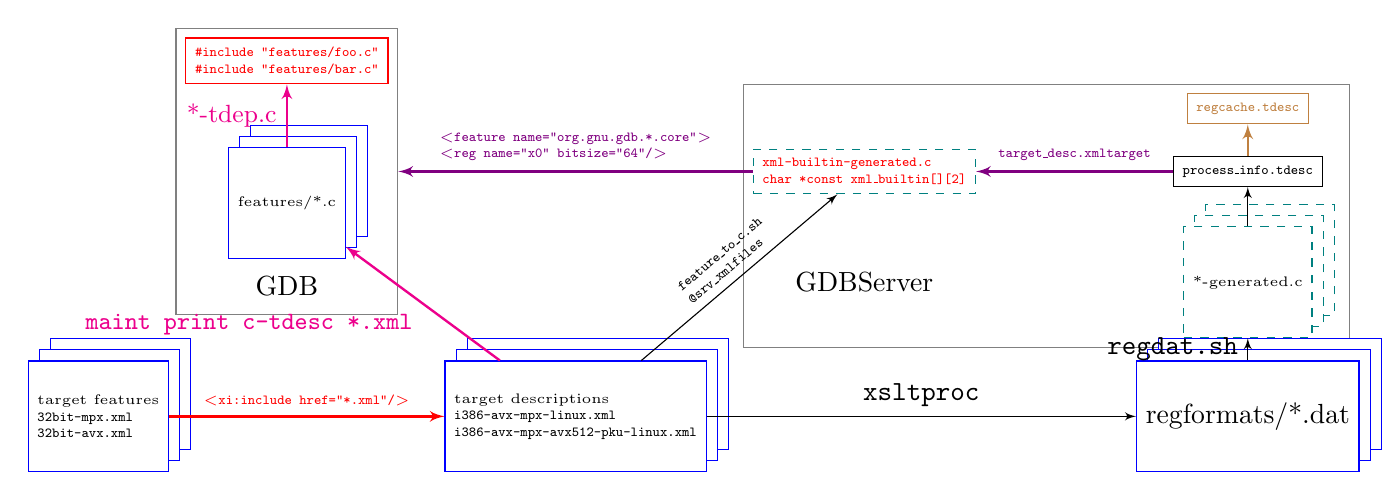
\begin{tikzpicture}[
  auto, >=latex',
  doc/.style={minimum height=4em, minimum width=3em, fill=white, draw=blue, double copy shadow={shadow xshift=4pt, 
      shadow yshift=4pt, fill=white, draw}},
]

  \node (gdb-tdep)[draw, align=left, font=\tiny, color=red] {\texttt{\#include "features/foo.c"}\\\texttt{\#include "features/bar.c"}};
  \node (gdb-features)[below=8mm of gdb-tdep, draw, align=left, doc] {\tiny features/*.c};
  \draw[->,color=magenta,line width=0.3mm] (gdb-features) -- node[align=left] {\small *-tdep.c} (gdb-tdep);
  \node (gdb) [below=1mm of gdb-features] {GDB};
  \node (gdb1) [draw=black!50, fit={(gdb) (gdb-tdep) (gdb-features) ($(gdb-features.south east)+(10pt,0pt)$)}] {};

  % GDBserver
  \node (gdbserver-builtin)[right=4.5cm of gdb1, align=left, draw=teal, dashed, font=\tiny, text=red] {\texttt{xml-builtin-generated.c} \\ \texttt{char *const xml\_builtin[][2]}};

  \node (gdbserver-process)[right=25mm of gdbserver-builtin, draw, align=left] {\tiny\texttt{process\_info.tdesc}};
  \node (gdbserver-generated)[below=5mm of gdbserver-process, align=left, doc, draw=teal, dashed] {\tiny *-generated.c};
  \node (gdbserver) [at=(gdbserver-builtin |- gdbserver-generated)] {GDBServer};
  \draw[->,color=violet,line width=0.3mm] (gdbserver-process) -- node[above,sloped]{\tiny\texttt{target\_desc.xmltarget}} (gdbserver-builtin);

  \node (gdbserver-regcache)[above=4mm of gdbserver-process,draw, align=left,color=brown] {\tiny\texttt{regcache.tdesc}};
  \draw[->] (gdbserver-generated) -- (gdbserver-process);
  \draw[->,color=brown,line width=0.3mm] (gdbserver-process) -- (gdbserver-regcache);
  \node (gdbserver1) [draw=black!50, fit={(gdbserver) (gdbserver-regcache) (gdbserver-process) (gdbserver-builtin) (gdbserver-generated) ($(gdbserver-generated.south east)+(10pt,0pt)$)}] {};
  \draw[->,color=violet,line width=0.3mm] (gdbserver-builtin) -- node[name=xml,align=left,sloped,font=\tiny] {\texttt{\textless feature name="org.gnu.gdb.*.core"\textgreater} \\ \texttt{\textless reg name="x0" bitsize="64"/\textgreater}} (gdb1);

  \node[below=2.4cm of xml, doc,align=left,font=\tiny] (doc) {target descriptions \\ \texttt{i386-avx-mpx-linux.xml} \\ \texttt{i386-avx-mpx-avx512-pku-linux.xml}};
  \node[left=35mm of doc, doc,align=left, anchor=east,font=\tiny] (features) {target features \\ \texttt{32bit-mpx.xml} \\ \texttt{32bit-avx.xml} };
  \draw[->,color=red,line width=0.3mm] (features) -- node {\tiny\texttt{\textless xi:include href="*.xml"/\textgreater}} (doc);

  \node[at=(gdbserver-generated |- doc), doc] (dat) {regformats/*.dat};

  \draw[->] (doc) -- node[above] {\texttt{xsltproc}} (dat);
  \draw[->] (dat) -- node {\texttt{regdat.sh}} (gdbserver-generated);
  \draw[->,color=magenta,line width=0.3mm] (doc) -- node[below, align=left, anchor=north east] {\small\texttt{maint print c-tdesc *.xml}} (gdb-features);
  \draw[->] (doc) -- node[above, align=left, sloped, font=\tiny] {\texttt{feature\_to\_c.sh} \\ \texttt{@srv\_xmlfiles}} (gdbserver-builtin);
\end{tikzpicture}

      \end{adjustbox}
      \caption{Existing design}
    \end{figure}

    \column[t]{0.5\textwidth}
    \begin{figure}[t]
      \centering
      \vspace*{-1cm}
      \begin{adjustbox}{precode=\dbox, max totalsize={1\textwidth},center}
        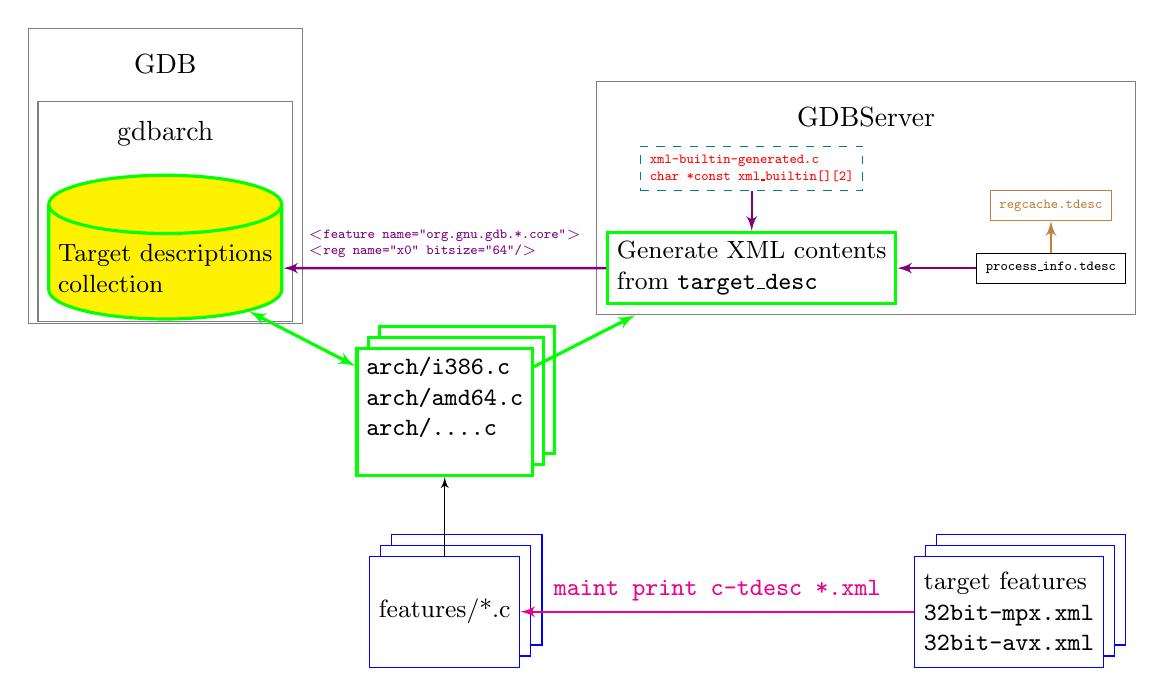
\begin{tikzpicture}[
  auto, >=latex',
  doc/.style={minimum height=4em, minimum width=3em, fill=white, draw=blue, double copy shadow={shadow xshift=4pt, 
      shadow yshift=4pt, fill=white, draw}},
  database/.style={cylinder, cylinder uses custom fill, cylinder body fill=yellow,
    cylinder end fill=yellow, shape border rotate=90, aspect=0.25,
    line width=0.4mm, draw=green
    }
]

  %\node (tdesc-collection) [database, left=4.5cm of gdbserver-builtin, font=\small, align=left] {Target descriptions\\collection};
  \node (tdesc-collection) [database, font=\small, align=left] {Target descriptions\\collection};
  \node (gdbarch) [above=1mm of tdesc-collection, draw=black!50, fit={($(tdesc-collection.north)+(0pt, 20pt)$) (tdesc-collection)}, label={[yshift=-20pt]gdbarch}]{};
  \node (gdb) [above=1mm of gdbarch, draw=black!50, fit={($(gdbarch.north)+(0pt, 20pt)$) (gdbarch)}, label={[yshift=-20pt]GDB}]{};


%($(gdb-features.south east)+(10pt,0pt)$)

  % GDBserver
  \node (gdbserver-gen-xml)[align=left, right=4.1cm of tdesc-collection,line width=0.4mm, draw=green, font=\small] {Generate XML contents \\from \texttt{target\_desc}};
  \node (gdbserver-builtin)[above=5mm of gdbserver-gen-xml, align=left, draw=teal, dashed, font=\tiny, text=red] {\texttt{xml-builtin-generated.c} \\ \texttt{char *const xml\_builtin[][2]}};

  \draw[->,color=violet,line width=0.3mm] (gdbserver-builtin) -- (gdbserver-gen-xml);


  \node (gdbserver-process)[right=of gdbserver-gen-xml, draw, align=left] {\tiny\texttt{process\_info.tdesc}};

  \draw[->,color=violet,line width=0.3mm] (gdbserver-process) -- (gdbserver-gen-xml);

  \node (gdbserver-regcache)[above=4mm of gdbserver-process,draw, align=left,color=brown] {\tiny\texttt{regcache.tdesc}};
  %\node (gdbserver) [at=(gdbserver-gen-xml |- gdbserver-regcache)] {GDBServer};

  \draw[->,color=brown,line width=0.3mm] (gdbserver-process) -- (gdbserver-regcache);
  \node (gdbserver1) [draw=black!50, fit={(gdbserver-regcache) (gdbserver-process) (gdbserver-gen-xml) (gdbserver-builtin) ($(gdbserver-builtin.north)+(0pt, 20pt)$)}, label={[yshift=-20pt]GDBServer}] {};



  \draw[->,color=violet,line width=0.3mm] (gdbserver-gen-xml) -- node[name=xml,align=left, sloped, font=\tiny] {\texttt{\textless feature name="org.gnu.gdb.*.core"\textgreater} \\ \texttt{\textless reg name="x0" bitsize="64"/\textgreater}} (tdesc-collection);

% \texttt{\textless feature name="org.gnu.gdb.*.core"\textgreater} \\ \texttt{\textless reg name="x0" bitsize="64"/\textgreater}

  \node (shared-tdesc)[below=of xml, draw, align=left, doc, font=\small, line width=0.4mm, draw=green] {
    \texttt{arch/i386.c} \\
    \texttt{arch/amd64.c} \\
    \texttt{arch/....c} \\
  };

  \draw[<->, line width=0.4mm, color=green] (shared-tdesc) -- (tdesc-collection);

  \draw[->, line width=0.4mm, color=green] (shared-tdesc) -- (gdbserver1);
  %\draw[->, line width=0.4mm, color=green] (shared-tdesc) -- (gdb1);

  \node (gdb-features)[below=of shared-tdesc, draw, align=left, doc] {\small features/*.c};

  \draw[->] (gdb-features) -- (shared-tdesc);

  \node[right=50mm of gdb-features, doc,align=left, font=\small] (features) {target features \\ \texttt{32bit-mpx.xml} \\ \texttt{32bit-avx.xml} };

  \draw[->,color=magenta,line width=0.3mm] (features) -- node[align=left, above] {\small\texttt{maint print c-tdesc *.xml}} (gdb-features);
\end{tikzpicture}

      \end{adjustbox}
      \caption{New design}
    \end{figure}
  \end{columns}

  \begin{columns}

    \column[t]{0.5\textwidth}
    \vspace*{-2cm}
    \only<3->{
      \begin{exampleblock}{Flexible target description creation}
        \begin{adjustbox}{max totalsize={1\textwidth}{1\textheight}, center}
          \lstinputlisting[language=C]{code/x86-tdesc.c}
        \end{adjustbox}
      \end{exampleblock}
    }


    \column[t]{0.5\textwidth}
    \vspace*{-0.5cm}

    \begin{block}{New design}
      {
        \only<+->{}
        \note<.>[item]{New diagram of new design, compared with the old one.  The new one is simpler than the old one.}
        \note<.>[item]{Something is removed, something is added,}
        \small
        \begin{itemize}
        \item<+-> No change in GDB remote protocol and target description specification,
          \note<.>{No compatibility issue}
        \item<+-> Flexible target description creation,
          \note<.>[item]{Generate *.c files from target features XML files instead of target description XML files,}
          \note<.>[item]{create target description in C, which is more flexible than xi:include in xml,}
        \item<+-> GDBserver generates XML contents for GDB's query, based on \texttt{xml\_builtin},
          \note<.>{xml\_builtin only contains features, reduce duplication.  Should be improved further, see TODO.}
        \end{itemize}
      }
    \end{block}
    \vspace*{-.5cm}
    
  \end{columns}
}

\subsection{Project status}

\frame{
  \frametitle{Implementation}

  \vspace*{-0.8cm}
  \begin{columns}[t]
    \begin{column}[t]{0.5\textwidth}

  \begin{itemize}
  \item<+-> Start from x86 target descriptions,
    \note<.>{to demonstrate the new approach of creating target descriptions in both GDB and GDBserver}
  \end{itemize}

  \end{column}

    \begin{column}[t]{0.5\textwidth}
      \begin{itemize}
      \item<+-> Target descriptions collection
        \begin{adjustbox}{max totalsize={.9\textwidth}}
          \lstinputlisting[language=C]{code/x86-tdesc-1.c}
        \end{adjustbox}
        \note<.>{easily create a collection of target descriptions}
      \end{itemize}
    \end{column}
  \end{columns}



  \begin{itemize}

  \item<+-> \texttt{xml\_builtin} is only for target features,

    \note<.>{The left is the old one, and the right side is new one,}
  \begin{columns}[t]
    \begin{column}[t]{.5\textwidth}
      \begin{adjustbox}{max totalsize={.8\textwidth},center}
        \lstinputlisting[language=C,caption=Old]{code/xml-builtin.c}
      \end{adjustbox}
    \end{column}

    \begin{column}[t]{.5\textwidth}
    \begin{adjustbox}{max totalsize={.9\textwidth},center}
      \lstinputlisting[language=C,caption=New]{code/xml-builtin-new.c}
    \end{adjustbox}
    \end{column}
  \end{columns}
  \end{itemize}
}

\frame{
  \frametitle{TODO and future work}

  \vspace*{-0.8cm}
  \begin{columns}[t]
    \begin{column}[t]{0.5\textwidth}

  \begin{itemize}
    \item<+-> \small Convert the rest (non-x86) target descriptions.  Helps are needed.
    \item<+-> \small Improve the XML generation in GDBserver.  GDBserver can only generate XML contents in the unit of target feature,
      \begin{adjustbox}{max totalsize={.8\textwidth},precode=\dbox,clip=true,
          trim={.35\width} % Trim width from the left
          {.60\height} % Trim height from the bottom
          {.10\width} % Trim width from the right
          {.15\height}} % Trim height from the top
        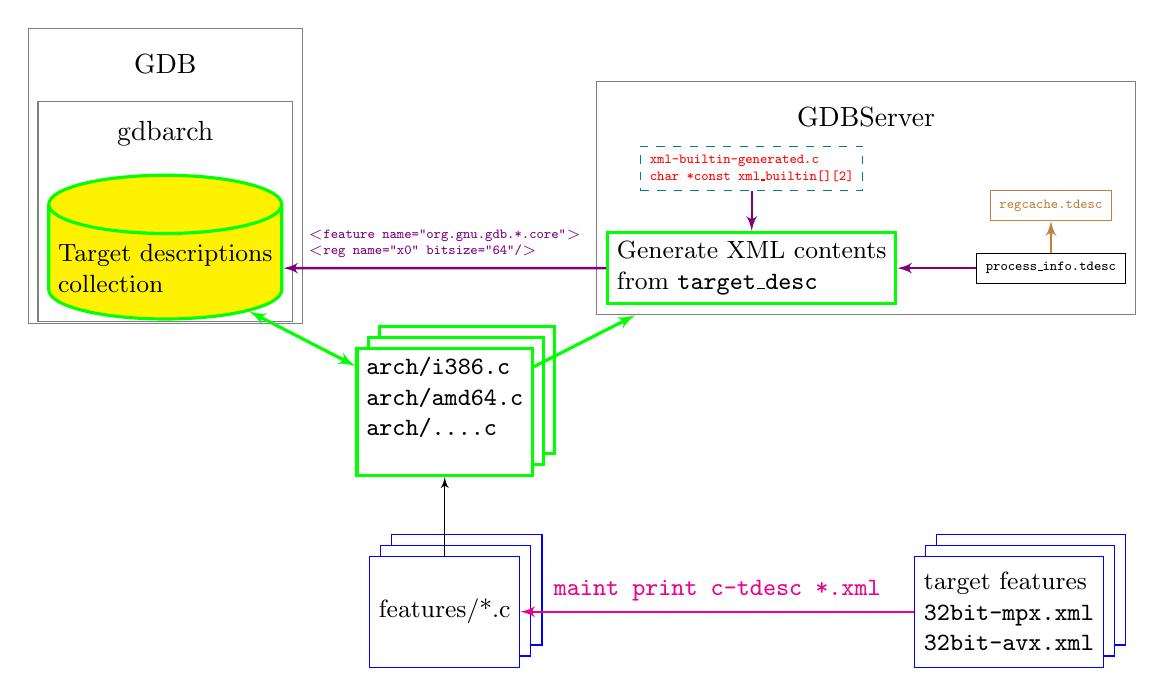
\begin{tikzpicture}[
  auto, >=latex',
  doc/.style={minimum height=4em, minimum width=3em, fill=white, draw=blue, double copy shadow={shadow xshift=4pt, 
      shadow yshift=4pt, fill=white, draw}},
  database/.style={cylinder, cylinder uses custom fill, cylinder body fill=yellow,
    cylinder end fill=yellow, shape border rotate=90, aspect=0.25,
    line width=0.4mm, draw=green
    }
]

  %\node (tdesc-collection) [database, left=4.5cm of gdbserver-builtin, font=\small, align=left] {Target descriptions\\collection};
  \node (tdesc-collection) [database, font=\small, align=left] {Target descriptions\\collection};
  \node (gdbarch) [above=1mm of tdesc-collection, draw=black!50, fit={($(tdesc-collection.north)+(0pt, 20pt)$) (tdesc-collection)}, label={[yshift=-20pt]gdbarch}]{};
  \node (gdb) [above=1mm of gdbarch, draw=black!50, fit={($(gdbarch.north)+(0pt, 20pt)$) (gdbarch)}, label={[yshift=-20pt]GDB}]{};


%($(gdb-features.south east)+(10pt,0pt)$)

  % GDBserver
  \node (gdbserver-gen-xml)[align=left, right=4.1cm of tdesc-collection,line width=0.4mm, draw=green, font=\small] {Generate XML contents \\from \texttt{target\_desc}};
  \node (gdbserver-builtin)[above=5mm of gdbserver-gen-xml, align=left, draw=teal, dashed, font=\tiny, text=red] {\texttt{xml-builtin-generated.c} \\ \texttt{char *const xml\_builtin[][2]}};

  \draw[->,color=violet,line width=0.3mm] (gdbserver-builtin) -- (gdbserver-gen-xml);


  \node (gdbserver-process)[right=of gdbserver-gen-xml, draw, align=left] {\tiny\texttt{process\_info.tdesc}};

  \draw[->,color=violet,line width=0.3mm] (gdbserver-process) -- (gdbserver-gen-xml);

  \node (gdbserver-regcache)[above=4mm of gdbserver-process,draw, align=left,color=brown] {\tiny\texttt{regcache.tdesc}};
  %\node (gdbserver) [at=(gdbserver-gen-xml |- gdbserver-regcache)] {GDBServer};

  \draw[->,color=brown,line width=0.3mm] (gdbserver-process) -- (gdbserver-regcache);
  \node (gdbserver1) [draw=black!50, fit={(gdbserver-regcache) (gdbserver-process) (gdbserver-gen-xml) (gdbserver-builtin) ($(gdbserver-builtin.north)+(0pt, 20pt)$)}, label={[yshift=-20pt]GDBServer}] {};



  \draw[->,color=violet,line width=0.3mm] (gdbserver-gen-xml) -- node[name=xml,align=left, sloped, font=\tiny] {\texttt{\textless feature name="org.gnu.gdb.*.core"\textgreater} \\ \texttt{\textless reg name="x0" bitsize="64"/\textgreater}} (tdesc-collection);

% \texttt{\textless feature name="org.gnu.gdb.*.core"\textgreater} \\ \texttt{\textless reg name="x0" bitsize="64"/\textgreater}

  \node (shared-tdesc)[below=of xml, draw, align=left, doc, font=\small, line width=0.4mm, draw=green] {
    \texttt{arch/i386.c} \\
    \texttt{arch/amd64.c} \\
    \texttt{arch/....c} \\
  };

  \draw[<->, line width=0.4mm, color=green] (shared-tdesc) -- (tdesc-collection);

  \draw[->, line width=0.4mm, color=green] (shared-tdesc) -- (gdbserver1);
  %\draw[->, line width=0.4mm, color=green] (shared-tdesc) -- (gdb1);

  \node (gdb-features)[below=of shared-tdesc, draw, align=left, doc] {\small features/*.c};

  \draw[->] (gdb-features) -- (shared-tdesc);

  \node[right=50mm of gdb-features, doc,align=left, font=\small] (features) {target features \\ \texttt{32bit-mpx.xml} \\ \texttt{32bit-avx.xml} };

  \draw[->,color=magenta,line width=0.3mm] (features) -- node[align=left, above] {\small\texttt{maint print c-tdesc *.xml}} (gdb-features);
\end{tikzpicture}

      \end{adjustbox}

      \begin{adjustbox}{max totalsize={.6\textwidth}}
        \lstinputlisting[language=XML,linerange=4-8,caption={Only xi:include features}]{code/aarch64.xml}
      \end{adjustbox}

      \begin{adjustbox}{max totalsize={.8\textwidth}}
        \lstinputlisting[language=XML,linerange=12-22,caption={More than xi:include features},
          linebackgroundcolor={
            \ifnum\value{lstnumber}>6
              \ifnum\value{lstnumber}<11\color{green}
              \fi
            \fi
        }]{code/s390-linux64.xml}
      \end{adjustbox}

      \note<.>[item]{GDBserver can only generate XML contents of using xi:include,}
      \note<.>[item]{It can't generate XML like s390,}

  \end{itemize}
      \end{column}

    \begin{column}[t]{0.55\textwidth}

      \begin{itemize}

    \item <+->\small Better resource management to \texttt{target\_desc},
      \begin{itemize}
        \item \small Automatically release \texttt{target\_desc} when it is not used,
        \item \small \texttt{target\_ops.to\_read\_description} return \texttt{std::shared\_ptr<target\_desc>}
      \end{itemize}
      \note<.>[item]{create different tdesc for different inferiors, after the inferiors are died, we don't have to keep all of them,}

    \item <+->\small target description changes in the runtime,
      \note<.>[item]{it is required actually many times, from different parts,}
      \begin{itemize}
        \item \small QEMU, target switching between AArch64 and AArch32,
        \item \small debugging Linux boot code, handling mode and bit width changes (16, 32 and 64),
          % https://sourceware.org/ml/gdb/2009-01/msg00008.html
          \note<.>{user has to manually \texttt{set arch}}
          % https://sourceware.org/bugzilla/show_bug.cgi?id=13984
        \item \small \href{https://sourceware.org/ml/gdb-patches/2016-06/msg00425.html}{MIPS: Handle run-time reconfigurable FPR size},
        \item ARM SVE vector registers,
      \end{itemize}


    \end{itemize}

    \end{column}
  \end{columns}
}

\section{End}
\frame{
  \frametitle{End}
}

\end{document}
